\section*{Scheduling Metric 1: Turnaround Time}
\begin{equation}
  \label{eq:turnaround}
  T_{\text{turnaround}} = T_{\text{completion}} - T_{\text{arrival}}
\end{equation}
\begin{minipage}{.5\linewidth}
\section*{FIFO or FCFS}
\begin{align*}
  T_{\text{arrival}}    & = 0 \\
  T_{\text{turnaround}} & = \frac{10+20+34}{3} = 3
\end{align*}
\end{minipage}
\begin{minipage}{.5\linewidth}
  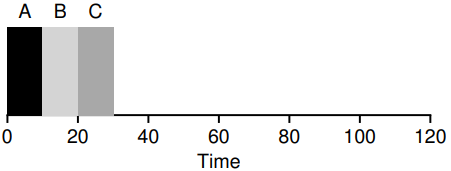
\includegraphics[width=\linewidth]{imgs/sched_fifo1}
\end{minipage}
\begin{minipage}{.5\linewidth}
short queued after long, bad
\begin{equation*}
  T_{\text{turnard}} = \frac{100+110+120}{3} = 110
\end{equation*}
\end{minipage}
\begin{minipage}{.5\linewidth}
  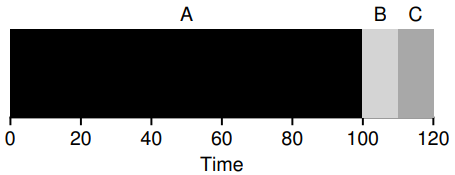
\includegraphics[width=\linewidth]{imgs/sched_fifo2}
\end{minipage}
% SJF
\begin{minipage}{.5\linewidth}
\section*{Shortest Job First (SJF)}
\begin{equation*}
  T_{\text{turnard}} = \frac{10+20+120}{3} = 50
\end{equation*}
\end{minipage}
\begin{minipage}{.5\linewidth}
  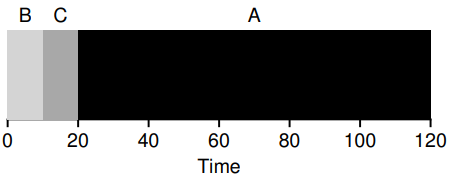
\includegraphics[width=\linewidth]{imgs/sched_fifo3}
\end{minipage}
\begin{minipage}{.5\linewidth}
  \begin{align*}
    & T_{\text{arrival-B}} = T_{\text{arrival-C}} = 10 \\
    & T_{t} = 103.33 = \\
    &\frac{100+(110-10)+(120-10)}{3} \\
  \end{align*}
\end{minipage}
\begin{minipage}{.5\linewidth}
  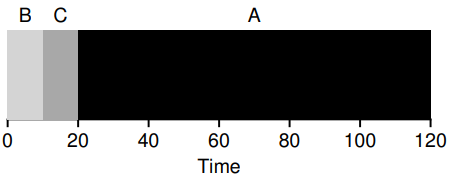
\includegraphics[width=\linewidth]{imgs/sched_fifo3}
\end{minipage}
\begin{minipage}{.5\linewidth}
  \begin{align*}
    & T_{t} = 50 = \\
    & \frac{(120-0)+(20-10)+(30-10)}{3} \\
  \end{align*}
\end{minipage}
\begin{minipage}{.5\linewidth}
  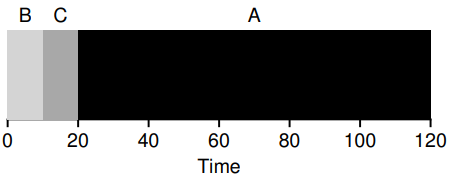
\includegraphics[width=\linewidth]{imgs/sched_fifo3}
\end{minipage}
\section*{Scheduling Metric 1: Response Time}
\begin{equation}
  \label{eq:reponse}
  T_{\text{response}} = T_{\text{firstrun}} - T_{\text{arrival}}
\end{equation}
\begin{minipage}{.5\linewidth}
  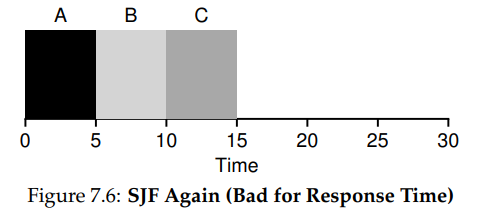
\includegraphics[width=\linewidth]{imgs/sched_rr1}
\end{minipage}
\begin{minipage}{.5\linewidth}
  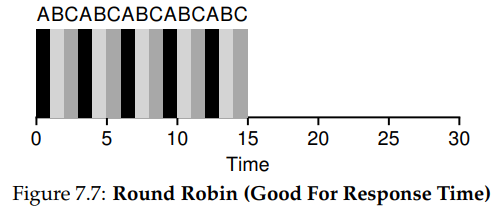
\includegraphics[width=\linewidth]{imgs/sched_rr}
\end{minipage}
\begin{minipage}{.5\linewidth}
  \centering
  SJF, $T_{r} = \frac{0+5+10}{3} = 5$
\end{minipage}
\begin{minipage}{.5\linewidth}
  RR (1s time slice), $T_{r} = \frac{0+1+2}{3} = 1$
\end{minipage}
\section*{Overlap improves resource usage}
\begin{minipage}{.45\linewidth}
  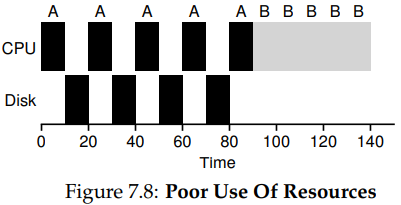
\includegraphics[width=\linewidth]{imgs/sched_io1}
\end{minipage}
\begin{minipage}{.55\linewidth}
  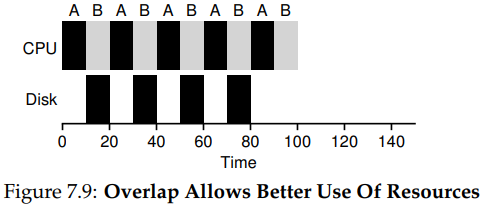
\includegraphics[width=\linewidth]{imgs/sched_io2}
\end{minipage}
\section*{MLFQ: Multi-Level Feedback Queue}
\begin{itemize}
\item \textbf{Rule 1}: if Priority(A) $>$ Priority(B), A runs (B doesn't)
\item \textbf{Rule 2}: if Priority(A) = Priority(B), A \& B runs in RR
\item \textbf{Rule 3}: When a job enters the system, it is placed at the \mo{highest} priority (the topmost queue)
\item \textbf{Rule 4}: Once a job uses up its time allotment at a given level (regardless of how many times it has given up the CPU), its priority is reduced (i.e., it moves down one queue)
\item \textbf{Rule 5}: After some time period S, move all the jobs in the system to the topmost queue.
\end{itemize}
\begin{minipage}{.4\linewidth}
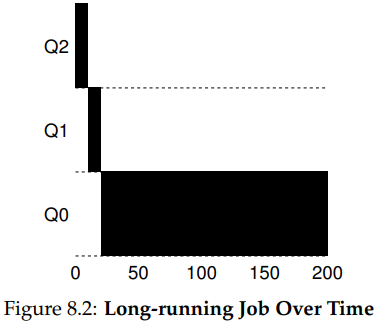
\includegraphics[width=\linewidth]{imgs/sched_longr}
\end{minipage}
\begin{minipage}{.6\linewidth}
  \flushleft
  \begin{itemize}
  \item assume time slice = 10 ms (with the allotment set equal to the time slice)
  \item the job enters at the highest priority (Q2)
  \item  After a single time slice of 10 ms, the scheduler reduces the job's priority by one, and thus the job is on Q1
  \item After running at Q1 for a time slice, the job is finally lowered to the lowest priority in the system (Q0), where it remains
  \end{itemize}
\end{minipage}
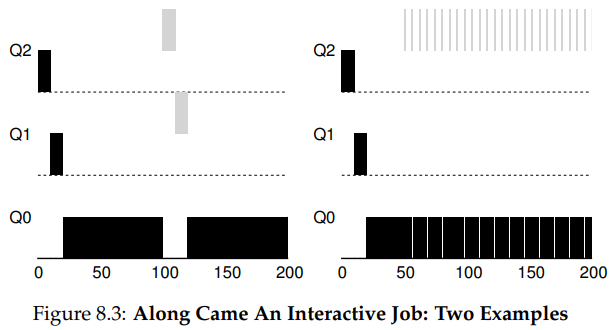
\includegraphics[width=\linewidth,height=3.5cm]{imgs/sched_long2}
\begin{minipage}{.5\linewidth}
  \flushleft
  \begin{itemize}
  \item  Job A (black) running along in the lowest-priority queue (as would any long-running CPU-intensive jobs)
  \item B (gray) arrives at time $T$ = 100; inserted into the highest queue
  \item B's short run-time: only 20 ms and completes before reaching the bottom queue in two time slices
  \item A resumes running (at low priority, as expected)
  \end{itemize}
\end{minipage}
\begin{minipage}{.5\linewidth}
  \flushleft
  \begin{itemize}
  \item interactive job B (gray) needs CPU only for 1ms before an I/O competing for CPU
  \item a long-running batch job A (shown in black)
  \item The MLFQ approach keeps B at the highest priority because B keeps releasing the CPU
  \item if B is an interactive job, MLFQ further achieves its goal of running interactive jobs quickly
  \end{itemize}
\end{minipage}
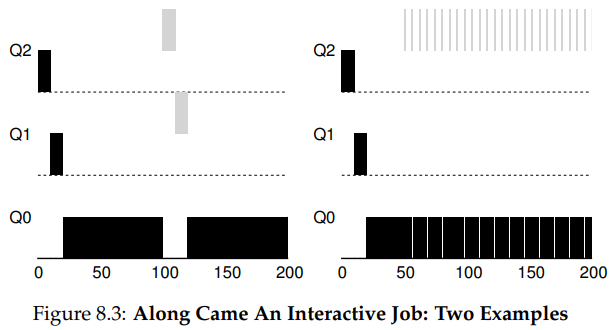
\includegraphics[width=\linewidth,height=3.5cm]{imgs/sched_long2}
\begin{minipage}{.5\linewidth}
  \flushleft
  \begin{itemize}
  \item there is no priority boost
  \item the long-running job gets starved once the two short jobs arrive
  \end{itemize}
\end{minipage}
\begin{minipage}{.5\linewidth}
  \flushleft
  \begin{itemize}
  \item there is a priority boost every 100ms (larger in real-world)
  \item long-running job gets boosted to the highest priority every 100ms
  \end{itemize}
\end{minipage}
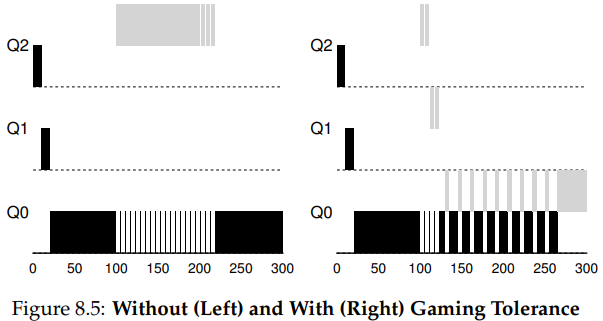
\includegraphics[width=\linewidth,height=3.5cm]{imgs/sched_g}
\begin{minipage}{.5\linewidth}
  \flushleft
  \begin{itemize}
  \item issue an I/O before proc's allotment ends $\to$ stay at same priority level; dominate CPU time
  \end{itemize}
\end{minipage}
\begin{minipage}{.5\linewidth}
  \flushleft
  \begin{itemize}
  \item regardless of the I/O behavior of proc, it slowly moves down the queues: \emph{cannot} dominate CPU
  \end{itemize}
\end{minipage}
\section*{Lottery Scheduler (need a random algorithm; has \emph{no} global state)}
\begin{minipage}{.75\linewidth}
\begin{lstlisting}[language=c]
// counter: used to track if we've found winner yet
int counter = 0;
// winner: call some random number generator to
// get a value >= 0 and <= (totaltickets - 1)
int winner = getrandom(0, totaltickets);
// current: use this to walk through the list of jobs
node_t *current = head; // best sorted HighT -> lowT
   while (current) {
   counter = counter + current->tickets;
   if (counter > winner)
      break; // found the winner
   current = current->next;
 }
 // `current' is the winner: schedule it...
\end{lstlisting}
\end{minipage}
\begin{minipage}{.25\linewidth}
  \flushleft
  \begin{itemize}
  \item probabilistic fairness, not deterministic
  \item scheduler must know total \# of tickets
  \item need data structs to track procs (e.g. list)
  \item for best efficiency, sort task-tickets from high to low
  \end{itemize}
\end{minipage}
\begin{minipage}{.45\linewidth}
  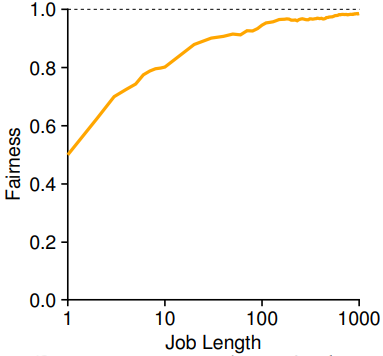
\includegraphics[width=\linewidth]{imgs/sched_lot_fair}
\end{minipage}
\begin{minipage}{.55\linewidth}
  \flushleft
  \begin{itemize}
  \item fairness metric $F = \frac{T_{\text{1st-job-done}}}{T_{\text{2nd-job-done}}}$
  \item for all jobs: same runtime $R$ and tickets (100)
  \item if $T_1 = 10$ $T_2 = 20$, $F = \frac{10}{20} = 0.5$
  \item if $T_1 = T_2 \to F = 1$, perfectly fair
  \item when job length not very long, average fairness quite low
  \item when jobs run for a significant number of time slices, lottery scheduler approach the desired fair outcome
  \end{itemize}
\end{minipage}
\section*{Linux Completely Fair Scheduler (CFS) and Weighting (Niceness)}
\begin{itemize}
\item goal: to fairly divide a CPU evenly among all competing processes
\item as each proc runs, \texttt{vruntime} $\uparrow$ at same rate, in proport.
with real time
\item when scheduling, CFS picks the proc with \mo{lowest} \texttt{vruntime} to run next
\item if CFS switch too often: fairness $\uparrow$, ctx switch cost $\uparrow$, performance $\downarrow$
\item CFS uses \texttt{sched\_latency} to decide length a proc runs before switch; typical 48ms and each proc runs 48/$n$ where $n=$ \# of procs
\item CFS uses \texttt{Min(sched\_latency, min\_granularity)} min defaults to 6ms to avoid large $n$ and tiny \texttt{sched\_latency} $\to$ close to 100\% fairness
\item CFS uses a \mo{periodic timer interrupt} $\to$ only make decisions at fixed time intervals (1ms); CFS tracks \texttt{vruntime} precisely: over the long haul, eventually approximate ideal sharing of the CPU
\end{itemize}
\begin{minipage}{.66\linewidth}
\begin{lstlisting}[language=c]
static const int prio_to_weight[40] = {
   /* -20 */ 88761, 71755, 56483, 46273, 36291,
   /* -15 */ 29154, 23254, 18705, 14949, 11916,
   /* -10 */ 9548, 7620, 6100, 4904, 3906,
   /*  -5  */ 3121, 2501, 1991, 1586, 1277,
   /*   0  */ 1024, 820, 655, 526, 423,
   /*   5  */ 335, 272, 215, 172, 137,
   /*  10  */ 110, 87, 70, 56, 45,
   /*  15  */ 36, 29, 23, 18, 15,
};
\end{lstlisting}
\end{minipage}
\begin{minipage}{.34\linewidth}
  \flushleft
  \begin{itemize}
  \item \mb{nice} level of a process $[-20, +19]$
  \item default nice = 0
  \item +nice $\to$ \mo{lower} priority
  \item -nice $\to$ \mo{higher} priority
  \item for each process: nice value \ding{220} \texttt{weight}
  \item preserves CPU proportion ratios
  \end{itemize}
\end{minipage}
\vspace{-.3em}
\begin{equation}
  \label{eq:timeslice}
  \texttt{time\_slice}_{k} = \frac{\texttt{weight}_{k}}{\sum_{i=0}^{n-1}\texttt{weight}_{i}}\cdot \texttt{sched\_latency}
\end{equation}
\begin{itemize}
\item jobs A (nice: -5) and B (nice: 0) $\to$ \texttt{weight}$_{A}$ = 3121; \texttt{weight}$_{B}$ = 1024
\item \texttt{time\_slice}$_{A} \approx \frac{3}{4}$ \texttt{sched\_latency} = 36ms; \texttt{time\_slice}$_{B} \approx 12$ms
\end{itemize}
\begin{equation}
  \label{eq:vruntime}
  \texttt{vruntime}_{i} = \texttt{vruntime}_{i} + \frac{\texttt{weight}_{0}}{\texttt{weight}_{i}}\cdot \texttt{runtime}_{i}
\end{equation}
\begin{itemize}
\item if nice$_{A}$ = 5, nice$_{B}$ = 10, CFS scheds them \emph{exactly} same as above
\item CFS uses a \ml{red}-black tree $O(\log(n))$: \emph{only} \mo{running} or \mo{runnable} procs kept therein; sleeping proc removed from the tree, tracked elsewhere
\item a job wakes, its \texttt{vruntime} sets to min value in the tree: no starvation
\item CFS can schedule across large groups of procs, not just individuals
\end{itemize}
